\documentclass{sbc2023}

\usepackage{graphicx}
\usepackage[misc,geometry]{ifsym}
\usepackage{fontspec}
\usepackage{fontawesome}
\usepackage{academicons}
\usepackage{color}
\usepackage{hyperref}
\usepackage{aas_macros}
\usepackage[bottom]{footmisc}
\usepackage{url}
\usepackage{multirow}
\usepackage{booktabs}
\usepackage{array}
\usepackage{tikz}
\usetikzlibrary{arrows.meta,positioning}

\setcitestyle{square}

\definecolor{darkblue}{rgb}{0.0,0.0,0.0}
\hypersetup{colorlinks,breaklinks,
            linkcolor=darkblue,urlcolor=darkblue,
            anchorcolor=darkblue,citecolor=darkblue}

\newcommand{\preencher}[1]{\textcolor{red}{[#1]}}
\renewenvironment{keywords}{\noindent\keywordfont{\textbf{Palavras-chave: }}}{\vskip6pt \rule{\linewidth}{.27pt}\vskip12pt}

\jid{Trabalho Prático}
\jtitle{Trabalho Prático de Computação Distribuída --- Ciência da Computação, PUC Minas, 2026/2}
\doi{}
\copyrightstatement{}
\jyear{2026}
\AtBeginDocument{\renewcommand{\refname}{Referências}\renewcommand{\figurename}{Figura}\renewcommand{\tablename}{Tabela}}

\title[Contagem distribuída de produtos em imagens]{Contagem distribuída de produtos em imagens: coordenação por web services e relógios lógicos de Lamport}

\author[Trabalho Prático --- Computação Distribuída]{
\affil{\textbf{André Vieira Penchel}, \textbf{Matheus Campello}, \textbf{João Vitor}, \textbf{Henrique Saldanha}, \textbf{Mateus Martins Parreiras} e \textbf{Arthur Campos}~~[~\textbf{PUC Minas}~]}
}

\begin{document}

\begin{frontmatter}
\maketitle

\begin{mail}
Instituto de Ciências Exatas e Informática, Pontifícia Universidade Católica de Minas Gerais, Belo Horizonte, MG, Brasil. Disciplina de Computação Distribuída, Prof. Luigi D. C. Soares. Primeira entrega.
\end{mail}

\begin{abstract}
\textbf{Resumo.~}
\noindent Este trabalho implementa um sistema distribuído que conta quantas unidades de um produto, descrito em linguagem natural (``garrafa de água''), aparecem em uma fotografia de prateleira ou estoque. A imagem é segmentada em superpixels com SLIC e cada superpixel é classificado pelo modelo CLIP, etapa cara em CPU. Uma API coordenadora corta a imagem em blocos sobrepostos, distribui os blocos por HTTP a dois ou mais workers que executam a segmentação e a classificação, costura as máscaras devolvidas e conta as instâncias. A comunicação entre os nós usa web services REST e todas as mensagens carregam carimbos de relógio lógico de Lamport, implementado manualmente, que permitem ordenar os eventos de envio e recepção entre máquinas sem depender de relógios físicos. O sistema foi executado em três máquinas virtuais na AWS provisionadas por Terraform, e o código, os testes e as instruções de execução estão em um repositório público no GitHub.
\end{abstract}

\begin{keywords}
Sistemas distribuídos, web services, relógio lógico de Lamport, segmentação de imagens, SLIC, CLIP
\end{keywords}

\end{frontmatter}


\section{O problema escolhido}
\label{sec:problema}

Escolhemos a sugestão de tema 3 do enunciado, segmentação de imagens distribuída com SLIC, aplicada a um problema concreto: dado o nome de um produto em português e uma foto de prateleira, armário ou estoque, responder quantas unidades daquele produto aparecem na foto. O usuário não precisa treinar nada nem cadastrar o produto antes; basta escrever o nome.

O algoritmo em uma única máquina funciona em quatro etapas. Primeiro a imagem é reduzida a no máximo 1000 pixels de lado e dividida em cerca de 600 superpixels com o SLIC \citep{achanta2012}, usando a implementação do scikit-image \citep{vanderwalt2014}. Em seguida, cada superpixel é recortado com uma janela de contexto e pontuado pelo CLIP \citep{radford2021}, um modelo que compara imagens e textos no mesmo espaço vetorial: frases como ``a photo of a water bottle on a store shelf'' são comparadas com as mesmas frases montadas para uma lista de negativos (``wooden shelf'', ``price tag'', ``cardboard box'', entre outros), e o superpixel recebe a probabilidade de ser o objeto procurado. Os superpixels acima de um limiar formam uma máscara binária, que passa por operações morfológicas. Por fim, a máscara é separada em instâncias com transformada de distância e \emph{watershed}, e as instâncias com área mínima são contadas e devolvidas com suas caixas delimitadoras.

A etapa do CLIP domina o custo: são centenas de inferências de uma rede neural por imagem, todas em CPU. Esse é o trabalho que dividimos entre máquinas. Como cada superpixel é classificado de forma independente, a imagem pode ser cortada em blocos e cada bloco processado por um nó diferente, o que caracteriza o problema como ``divisível em várias unidades de trabalho executadas de maneira distribuída'', como pede o enunciado.

\section{Arquitetura do sistema}
\label{sec:arquitetura}

O sistema tem três tipos de entidade, ilustrados na Figura~\ref{fig:arquitetura}.

\begin{figure}[t]
\centering
\resizebox{\linewidth}{!}{%
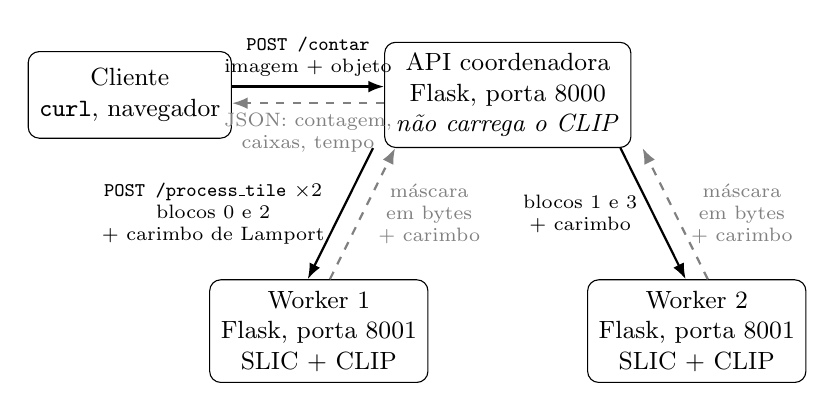
\begin{tikzpicture}[
  no/.style={draw,rounded corners,align=center,minimum height=1.1cm,font=\small,inner sep=4pt},
  seta/.style={-{Latex[length=2mm]},thick},
  volta/.style={-{Latex[length=2mm]},thick,dashed,gray},
  rot/.style={font=\scriptsize,align=center}
]
\node[no] (cli) at (0,0) {Cliente\\\texttt{curl}, navegador};
\node[no] (api) at (4.8,0) {API coordenadora\\Flask, porta 8000\\\emph{não carrega o CLIP}};
\node[no] (w1) at (2.4,-3.0) {Worker 1\\Flask, porta 8001\\SLIC + CLIP};
\node[no] (w2) at (7.2,-3.0) {Worker 2\\Flask, porta 8001\\SLIC + CLIP};
\draw[seta] ([yshift=3pt]cli.east) -- node[rot,above]{\texttt{POST /contar}\\imagem + objeto} ([yshift=3pt]api.west);
\draw[volta] ([yshift=-3pt]api.west) -- node[rot,below]{JSON: contagem,\\caixas, tempo} ([yshift=-3pt]cli.east);
\draw[seta] ([xshift=-4pt]api.south west) -- node[rot,left,xshift=-2pt]{\texttt{POST /process\_tile} $\times$2\\blocos 0 e 2\\+ carimbo de Lamport} ([xshift=-4pt]w1.north);
\draw[volta] ([xshift=4pt]w1.north) -- node[rot,right,xshift=2pt]{máscara\\em bytes\\+ carimbo} ([xshift=4pt]api.south west);
\draw[seta] ([xshift=-4pt]api.south east) -- node[rot,left,xshift=-2pt]{blocos 1 e 3\\+ carimbo} ([xshift=-4pt]w2.north);
\draw[volta] ([xshift=4pt]w2.north) -- node[rot,right,xshift=2pt]{máscara\\em bytes\\+ carimbo} ([xshift=4pt]api.south east);
\end{tikzpicture}}
\caption{Entidades e mensagens. A API corta a imagem em 4 blocos, envia dois para cada worker em paralelo e costura as máscaras devolvidas. Toda mensagem leva um carimbo de Lamport.}
\label{fig:arquitetura}
\end{figure}

\paragraph{Cliente.} Qualquer programa capaz de fazer uma requisição HTTP: usamos \texttt{curl} nos testes, mas a API libera CORS para ser chamada de um navegador. O cliente envia a foto e o nome do produto e recebe um JSON.

\paragraph{API coordenadora.} É o nó que conhece o problema inteiro, mas não executa a parte pesada: ela não carrega o modelo CLIP. Ao receber \texttt{POST /contar}, ela valida os parâmetros, reduz a imagem, corta-a em uma grade $2\times2$ com 20\% de sobreposição entre blocos vizinhos (para que um produto na fronteira não seja cortado ao meio), e despacha os blocos em paralelo, alternando entre os workers: blocos 0 e 2 vão para o primeiro, 1 e 3 para o segundo. Cada bloco recebe uma quantidade de superpixels proporcional à sua área, para que o tamanho médio de um superpixel seja o mesmo da versão em uma máquina. Quando as quatro máscaras voltam, a API copia apenas a zona central de cada uma para uma máscara global do tamanho da imagem, descartando as margens sobrepostas, e executa a separação e a contagem de instâncias localmente, pois essa etapa é barata e precisa da imagem inteira. Se qualquer bloco falhar, a resposta é HTTP 503 com a lista dos blocos que falharam; nunca devolvemos uma contagem parcial, que seria um resultado errado disfarçado de certo.

\paragraph{Workers.} São processos idênticos e sem estado, cada um em uma máquina, que carregam o CLIP uma única vez ao subir e atendem \texttt{POST /process\_tile}. Um worker não sabe de que imagem o bloco veio nem quantos workers existem; ele só segmenta, classifica e devolve a máscara.

A Tabela~\ref{tab:mensagens} resume quem fala com quem e o conteúdo de cada mensagem. A máscara é devolvida como bytes crus (um byte 0 ou 1 por pixel, tipo \texttt{application/octet-stream}) em vez de JSON: para um bloco de $600\times600$ pixels isso são 360~KB, contra vários megabytes se fosse uma lista JSON.

\begin{table}[t]
\caption{Mensagens trocadas entre as entidades.}
\label{tab:mensagens}
\footnotesize
\begin{tabular}{@{}>{\raggedright\arraybackslash}p{2.35cm}>{\raggedright\arraybackslash}p{5.6cm}@{}}
\toprule
\textbf{Mensagem} & \textbf{Conteúdo} \\
\midrule
Cliente $\to$ API \newline \texttt{POST /contar} & multipart: \texttt{imagem} (arquivo), \texttt{objeto} (texto) e parâmetros opcionais (\texttt{limiar}, \texttt{segmentos}, \ldots). \\
\addlinespace
API $\to$ Cliente & JSON: \texttt{quantidade}, lista de \texttt{instancias} com caixa, centro e área em pixels da imagem original, \texttt{tempo\_ms}. \\
\addlinespace
API $\to$ Worker \newline \texttt{POST} \newline \texttt{/process\_tile} & multipart: bloco em JPEG, \texttt{objeto}, \texttt{limiar}, \texttt{segmentos}, \texttt{compacidade}, \texttt{janela}; cabeçalhos \texttt{X-Task-Id} e \texttt{X-Lamport-Timestamp}. \\
\addlinespace
Worker $\to$ API & máscara binária em bytes (\texttt{application/octet-stream}); cabeçalhos \texttt{X-Task-Id}, \texttt{X-Lamport-Timestamp} e \texttt{X-Worker-Id}. \\
\addlinespace
API $\to$ Worker \newline \texttt{GET /health} & sem corpo; a API consolida o estado de cada worker no seu próprio \texttt{GET /health} (\texttt{ok} ou \texttt{degradado}). \\
\bottomrule
\end{tabular}
\end{table}

\section{Requisitos implementados}
\label{sec:requisitos}

Dos requisitos listados para a primeira entrega, implementamos dois: utilização de web services e sincronização de relógios lógicos.

\subsection{Web services}

Toda a comunicação entre os nós é feita por HTTP, no estilo REST, com o microframework Flask no lado servidor e a biblioteca \texttt{requests} no lado cliente. O enunciado permite bibliotecas para a comunicação, então o que é ``de prateleira'' aqui é o transporte HTTP; o protocolo de aplicação foi definido por nós: as rotas, os campos de cada mensagem, os cabeçalhos de identificação de tarefa e de relógio, a regra de despacho alternado, a sobreposição dos blocos e a costura das máscaras.

Escolhemos web services em vez de gRPC por três motivos. O primeiro é a facilidade de teste e demonstração: qualquer rota pode ser exercitada com \texttt{curl} ou de um navegador, sem gerar código a partir de um arquivo \texttt{.proto}. O segundo é que o produto final é uma API que um front-end chamaria diretamente, então o cliente já falaria HTTP de qualquer forma. O terceiro é a simplicidade de depuração: as mensagens entre API e workers são legíveis nos logs de cada máquina.

A API expõe quatro rotas. \texttt{POST /contar} é a principal e devolve o JSON descrito na Tabela~\ref{tab:mensagens}. \texttt{POST /contar/figura} recebe a mesma entrada e devolve um PNG com a foto, a máscara costurada e as instâncias numeradas, útil para conferir o resultado visualmente. \texttt{GET /objetos} lista os nomes em português que a API traduz para inglês antes de montar as frases do CLIP. \texttt{GET /health} consulta o \texttt{/health} de cada worker e responde \texttt{ok} ou \texttt{degradado}. O worker expõe \texttt{POST /process\_tile} e \texttt{GET /health}. Entradas inválidas (imagem vazia, limiar fora de $[0,1]$, arquivo acima de 20~MB) são recusadas com 400 ou 413 antes de qualquer envio aos workers, e o worker recusa com 422 uma requisição sem os cabeçalhos obrigatórios.

Os quatro blocos são enviados ao mesmo tempo, com um \emph{pool} de threads na API, e cada envio tem um tempo limite configurável (padrão de 300~s). Como os workers são sem estado, o endereço deles é apenas uma lista na variável de ambiente \texttt{WORKER\_URLS}; adicionar uma terceira máquina é acrescentar uma URL.

\subsection{Relógio lógico de Lamport}

Cada nó mantém um relógio lógico de Lamport \citep{lamport1978}: um contador inteiro que começa em zero. Implementamos as duas regras manualmente, sem biblioteca, em um módulo de 25 linhas protegido por uma trava, já que a API e os workers atendem várias requisições em threads concorrentes:

\begin{itemize}
\item \textbf{Evento local ou envio:} \texttt{tick()} incrementa o contador e devolve o novo valor, que vai no cabeçalho \texttt{X-Lamport-Timestamp} da mensagem.
\item \textbf{Recepção:} \texttt{receive(remoto)} faz $C \leftarrow \max(C, C_{remoto}) + 1$.
\end{itemize}

Na API, cada bloco despachado é um envio (\texttt{tick}) e cada resposta recebida, inclusive de erro, é uma recepção. No worker, a chegada de um bloco é uma recepção e a resposta é um envio; o carimbo do worker volta no cabeçalho da resposta, de modo que a API avança seu relógio ao receber. O identificador da tarefa (\texttt{X-Task-Id}, formado por um identificador do pedido mais o índice do bloco) acompanha o carimbo para que os eventos de uma mesma requisição possam ser correlacionados nos logs das três máquinas. O trecho abaixo, abreviado, é do log real do primeiro teste na AWS, com a API em uma máquina e o worker 1 em outra:

{\scriptsize
\begin{verbatim}
[api]     SEND    task=t0 worker=172.31.10.180 lamport=1
[api]     SEND    task=t1 worker=172.31.11.218 lamport=2
[api]     SEND    task=t2 worker=172.31.10.180 lamport=3
[api]     SEND    task=t3 worker=172.31.11.218 lamport=4
[worker1] RECEIVE task=t0 remote=1 lamport=2
[worker1] RECEIVE task=t2 remote=3 lamport=4
[worker1] SEND    task=t0 lamport=13
\end{verbatim}}

O worker 1 recebeu \texttt{t0} com carimbo remoto 1 e passou a 2; recebeu \texttt{t2} com carimbo 3 e passou a 4, mesmo que seu próprio relógio estivesse atrás (o salto até 13 vem de linhas omitidas, em que ele recebeu os blocos de um segundo pedido). Sem consultar os relógios físicos das duas máquinas, a cadeia de mensagens mostra que o envio de \texttt{t0} pela API (1) precede sua recepção no worker (2), que precede a resposta (13). Os carimbos sozinhos garantem apenas a relação inversa: um evento de carimbo maior nunca precede causalmente um de carimbo menor, logo a resposta não pode ter precedido nenhum dos quatro envios. Carimbo menor não implica ``aconteceu antes'': o envio de \texttt{t1} na API e a recepção de \texttt{t0} no worker 1 têm o mesmo carimbo 2 e são concorrentes, assim como os envios ao worker 2 são concorrentes com o processamento no worker 1. O relógio de Lamport dá só uma ordem parcial, e isso é esperado. O que o sistema ganha é uma forma de ordenar causalmente os eventos de cada requisição nos logs, detectar uma resposta que chegue com carimbo menor do que o esperado e, na segunda entrega, basear nele o tratamento de respostas atrasadas e reenvios.

\section{Execução e evidências}
\label{sec:execucao}

O código está no repositório público do grupo no GitHub\footnote{\url{https://github.com/Matheuscamp29/Trabalho-Computacao-Distribuida}}, ramo \texttt{main}; este relatório descreve o \emph{commit} \texttt{5cc3b8f}, de 1º de novembro de 2026. O \texttt{README} traz as instruções de execução, e há 12 testes unitários (\texttt{python -m unittest}) que exercitam a API, o despacho, a costura e o relógio lógico sem carregar o modelo, usando workers falsos.

\paragraph{Em uma máquina, para desenvolvimento.} Três terminais na raiz do repositório, com as dependências instaladas:

{\scriptsize
\begin{verbatim}
PORT=8001 WORKER_ID=worker1 python -m distribuido.worker
PORT=8002 WORKER_ID=worker2 python -m distribuido.worker
python api.py
\end{verbatim}}

\noindent A API procura os workers em \texttt{localhost}, portas 8001 e 8002, por padrão; em máquinas da mesma rede local basta apontar \texttt{WORKER\_URLS} para os IPs delas.

\paragraph{Em máquinas separadas, na AWS.} Para cumprir o requisito de nós em máquinas distintas, escrevemos a infraestrutura como código na pasta \texttt{infra/}, com Terraform. Um \texttt{terraform apply} cria cinco recursos na região \texttt{us-east-2}: o par de chaves SSH, um grupo de segurança que libera a porta 8000 apenas para o IP do grupo e a porta 8001 apenas entre as máquinas do próprio grupo, duas instâncias \texttt{t3.medium} (2 vCPUs, 4~GB) para os workers e uma \texttt{t3.small} para a API, todas com Ubuntu 24.04. Um \emph{script} de inicialização, executado pela própria AWS no primeiro boot, clona o repositório, instala as dependências e registra um serviço do sistema que sobe o worker ou a API com as variáveis de ambiente certas; o Terraform preenche \texttt{WORKER\_URLS} da API com os IPs internos dos workers. Nada é configurado manualmente nas máquinas.

Na execução de 1º de novembro de 2026, as máquinas receberam os endereços 18.119.119.159 (API), 3.15.11.21 e 18.119.115.239 (workers; 172.31.10.180 e 172.31.11.218 na rede interna). O \texttt{/health} consultado do computador do grupo respondeu:

{\scriptsize
\begin{verbatim}
{"status":"ok","workers":{"http://172.31.10.180:8001":true,
                          "http://172.31.11.218:8001":true}}
\end{verbatim}}

e a contagem de ``garrafa de agua'' na imagem \texttt{imagens/images.jpg} do repositório, enviada por \texttt{curl}, devolveu 4 instâncias com suas caixas em 38{,}6~s (\texttt{tempo\_ms} de 38633), com os quatro blocos processados por dois workers em máquinas diferentes. O custo das três máquinas é de cerca de US\$~0,12 por hora, e elas são destruídas com \texttt{terraform destroy} ao fim de cada sessão de testes, então os endereços acima não permanecem ativos; a execução pode ser repetida com qualquer conta da AWS seguindo o \texttt{README}.

\paragraph{Como verificar.} Com o sistema no ar, em qualquer das formas, três comandos reproduzem as evidências deste relatório, trocando \texttt{ENDERECO} pelo da API:

{\scriptsize
\begin{verbatim}
curl http://ENDERECO:8000/health
curl -F "imagem=@imagens/images.jpg" \
     -F "objeto=garrafa de agua" http://ENDERECO:8000/contar
ssh ubuntu@IP_DO_WORKER 'journalctl -u contador -f'
\end{verbatim}}

\noindent O terceiro mostra, ao vivo, as linhas \texttt{RECEIVE} e \texttt{SEND} com os carimbos de Lamport no worker enquanto o segundo é executado; em uma execução local, as mesmas linhas aparecem no terminal de cada processo.

\IfFileExists{figura_aws.png}{%
\begin{figure}[t]
\centering
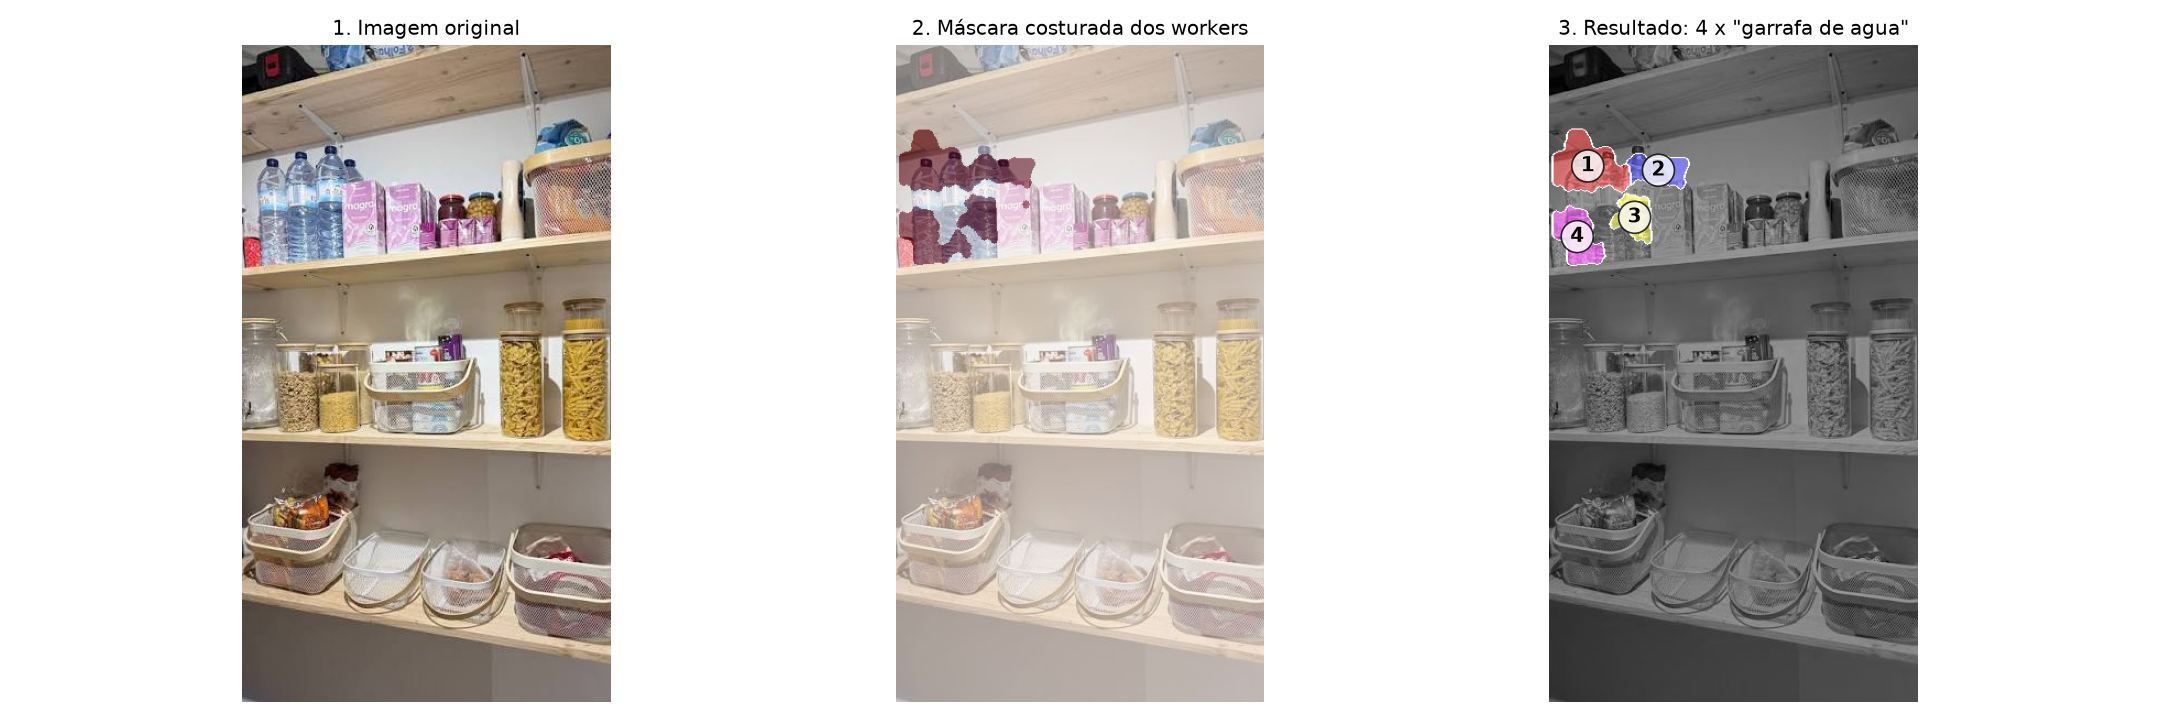
\includegraphics[width=\linewidth]{figura_aws.png}
\caption{Saída de \texttt{POST /contar/figura} na AWS para ``garrafa de agua'': foto original, máscara costurada a partir dos quatro blocos e instâncias numeradas.}
\label{fig:resultado}
\end{figure}}{}

\section{Desafios e problemas encontrados}
\label{sec:desafios}

\paragraph{Contexto perdido nas bordas.} O CLIP decide olhando o entorno de cada superpixel. Cortar a imagem em blocos sem sobreposição fazia produtos na fronteira serem classificados com metade do contexto e, muitas vezes, perdidos. A sobreposição de 20\% e a costura apenas da zona central resolveram o caso da borda, mas um bloco ainda vê menos imagem do que a versão em uma máquina, e a contagem distribuída pode diferir da local na mesma foto. Esse é o principal ponto a investigar na análise de desempenho da segunda entrega.

\paragraph{Trabalho repetido por bloco.} Na primeira versão a API repassava \texttt{segmentos=600} a cada bloco, o que gerava quatro vezes mais superpixels, e portanto quatro vezes mais inferências do CLIP, do que a versão local. Em um \emph{notebook} isso passava despercebido; nas instâncias \texttt{t3.medium} cada bloco levava mais de 150~s e a API, que esperava 60~s, respondia 503 em todos os pedidos. Diagnosticamos pelos logs das duas máquinas (o worker registrava a resposta com código 200 mais de um minuto depois de a API ter desistido) e corrigimos distribuindo os superpixels proporcionalmente à área: o tempo por imagem caiu para 38{,}6~s.

\paragraph{Simplicidade do código.} A primeira implementação da API usava recursos que dificultavam a leitura e a apresentação (decoradores de ciclo de vida, geradores, classes para configuração). Reescrevemos tudo em Flask com funções simples, uma rota por função e o relógio lógico como um módulo de estado global protegido por trava. O comportamento foi conferido comparando os resultados numéricos das duas versões nas imagens de exemplo.

\paragraph{Ambiente de nuvem.} A conta da AWS usada pelo grupo é do novo modelo de cadastro da AWS, que fixa a região do projeto por uma política da organização. O primeiro \texttt{terraform plan} em \texttt{us-east-1} falhou com ``explicit deny in a service control policy'' mesmo com o usuário tendo permissão de administrador; a causa só ficou clara na documentação da AWS, e a solução foi parametrizar a região e usar \texttt{us-east-2}.

\section{Papel de cada aluno}
\label{sec:papeis}

\begin{itemize}
\item \textbf{Matheus Campello:} pipeline de visão em uma máquina (14/10): segmentação SLIC, pontuação dos superpixels com o CLIP e as frases positivas e negativas, máscara com operações morfológicas, separação de instâncias por \emph{watershed} e contagem, tradução dos nomes de produto, figura de saída e imagens de exemplo.
\item \textbf{Mateus Martins Parreiras:} primeira versão da execução distribuída (19/10): corte da imagem em blocos com sobreposição, gerente que despacha os blocos e costura as máscaras, e o processo worker.
\item \textbf{Arthur Campos:} relógio lógico de Lamport (19/10): módulo do relógio, cabeçalhos \texttt{X-Task-Id} e \texttt{X-Lamport-Timestamp}, logs de envio e recepção, configuração com dois workers e os testes unitários do despacho, do relógio e do protocolo do worker.
\item \textbf{João Vitor:} rotas da API (\texttt{/contar}, \texttt{/contar/figura}, \texttt{/objetos} e \texttt{/health}), validação das entradas com os códigos de erro e documentação de execução no \texttt{README}.
\item \textbf{Henrique Saldanha:} infraestrutura na AWS: Terraform em \texttt{infra/}, \emph{script} de inicialização das máquinas com o serviço do sistema, subida e teste das três instâncias.
\item \textbf{André Vieira Penchel:} reescrita da API e dos workers em Flask com o código organizado em pastas (30/10), diagnóstico e correção do tempo limite e dos superpixels por bloco na AWS (01/11), coleta das evidências e redação do relatório.
\end{itemize}

\section{Conclusão e próximos passos}

O sistema cumpre os requisitos da primeira entrega com dois nós de processamento em máquinas distintas, comunicação por web services e relógios lógicos de Lamport implementados manualmente, e foi executado de ponta a ponta na AWS. Para a segunda entrega, o tratamento de falhas vai além do tempo limite atual: reenvio de um bloco ao outro worker quando o primeiro falha, verificação de saúde antes do despacho e tolerância à queda de um worker durante o processamento. A análise de desempenho comparará, no mesmo hardware, a execução em uma máquina com a distribuída, medindo tempo e diferença de contagem para as mesmas fotos.

\bibliographystyle{apalike-sol}
\bibliography{refs}

\end{document}
